\title{Particles and Plasma in Cosmological Evolution}

\author{
Jeremiah Birrell\inst{1}\fnmsep\thanks{\email{jeremey.birrell@gmail.com}},
Christopher Grayson\inst{1}\fnmsep\thanks{\email{chrisgray1044@arizona.edu}},
Johann Rafelski\inst{1}\fnmsep\thanks{\email{johannr@arizona.edu}}
Andrew Steinmetz\inst{1,2}\fnmsep\thanks{\email{ajsteinmetz@arizona.edu}},
Cheng Tao Yang\inst{1}\fnmsep\thanks{\email{chengtaoyang@arizona.edu}},
}

\institute{Department of Physics, The University of Arizona, Tucson, AZ, 85721, USA
\and Arizona College of Technology, Hebei University of Technology, Tianjin 300130, China
}

\abstract{
% Cheng Tao's Abstract
This work aims to deepen the understanding of the primordial composition of the Universe in the temperature range $300\,\mathrm{MeV}>T>0.02\,\mathrm{MeV}$. In the following I exploit known properties of elementary particles and apply methods of kinetic theory and statistical physics to advance the understanding of  the  cosmic plasma. Within the Big Bang model the Universe began as a highly energetic fireball with an immensely high temperature and energy density. Consequently, an ultra-relativistic plasma was generated, exhibiting distinct properties as the Universe expanded and cooled.  When the Universe is hot and dense, fundamental particles (such as quarks, leptons, and gauge bosons) play a crucial role in understanding the early Universe. These elementary particles were abundantly present once the temperature dropped below $T=130$\,GeV. Their interactions governed the dynamics of the early Universe. Our research focuses on investigation of these fundamental particles during the epoch which transits from primordial quark-gluon degrees of freedom to the era of normal matter plasma (H$^+$, He$^{+}$, $e^-$). Our findings will offer valuable insights into the properties of the early Universe governing the properties of matter surrounding us today.
% Jeremey's Abstract
% Chris's Abstract
% Andrew's Abstract (Needs revision!)
An interesting application of these theoretical developments is to study primordial magnetization in the early universe during the hot dense electron-positron plasma epoch. We propose a model of magnetic thermal matter-antimatter plasmas. We analyze the paramagnetic characteristics of electron-positron plasma when exposed to an external primordial field. We determine the magnitude of a small polarization asymmetry sufficient to generate field strengths in agreement with those measured today in deep intergalactic space.
} 
\maketitle
\setcounter{tocdepth}{2}
\tableofcontents

%%%%%%%%%%%%%%%%%%%%%%%%%%%%%%%%%%%%%%%
\section{Cosmology introduction}
\label{sec:flrw}
%%%%%%%%%%%%%%%%%%%%%%%%%%%%%%%%%%%%%%%
\noindent This section introduces some necessary concepts which will be useful in describing the magnetization of the electron-positron primordial plasma in \rchap{chap:cosmo}. We operate under the $\Lambda$ Cold Dark Matter $(\Lambda\mathrm{CDM})$ model of cosmology where the contemporary universe is approximately 69\% dark energy, 26\% dark matter, 5\% baryons, and $<1$\% photons and neutrinos in energy density~\cite{Davis:2003ad,Planck:2018vyg}. The standard picture of the universe's evolution is outlined in \rf{fig:cosmo}.

The Friedmann-Lema{\^i}tre-Robertson-Walker (FLRW) line element and metric~\cite{weinberg1972gravitation} in spherical coordinates is
\begin{gather}
    \label{FLRW} ds^2=dt^2-a^2(t)\left[\frac{dr^2}{1-kr^{2}}+r^{2}d\theta^2+r^{2}\sin\theta^{2}d\phi^2\right]\,,\\
    g_{\alpha\beta}=
    \begin{pmatrix}
        1&0&0&0\\
        0&-\frac{a^{2}(t)}{1-kr^{2}}&0&0\\
        0&0&-a^{2}(t)r^{2}&0\\
        0&0&0&-a^{2}(t)r^{2}\sin\theta^{2}
    \end{pmatrix}\,.
\end{gather}
The Gaussian curvature $k$ informs the spatial shape of the universe with the following possibilities: infinite flat Euclidean $(k=0)$, finite spherical but unbounded $(k=+1)$, or infinite hyperbolic saddle-shaped $(k=-1)$. Observation indicates our universe is flat or nearly so.

%%%%%%%%%%%%%%%%%%%%%%%%%%%%%%%%%%%%%%%
\begin{figure}[ht]
 \centering
 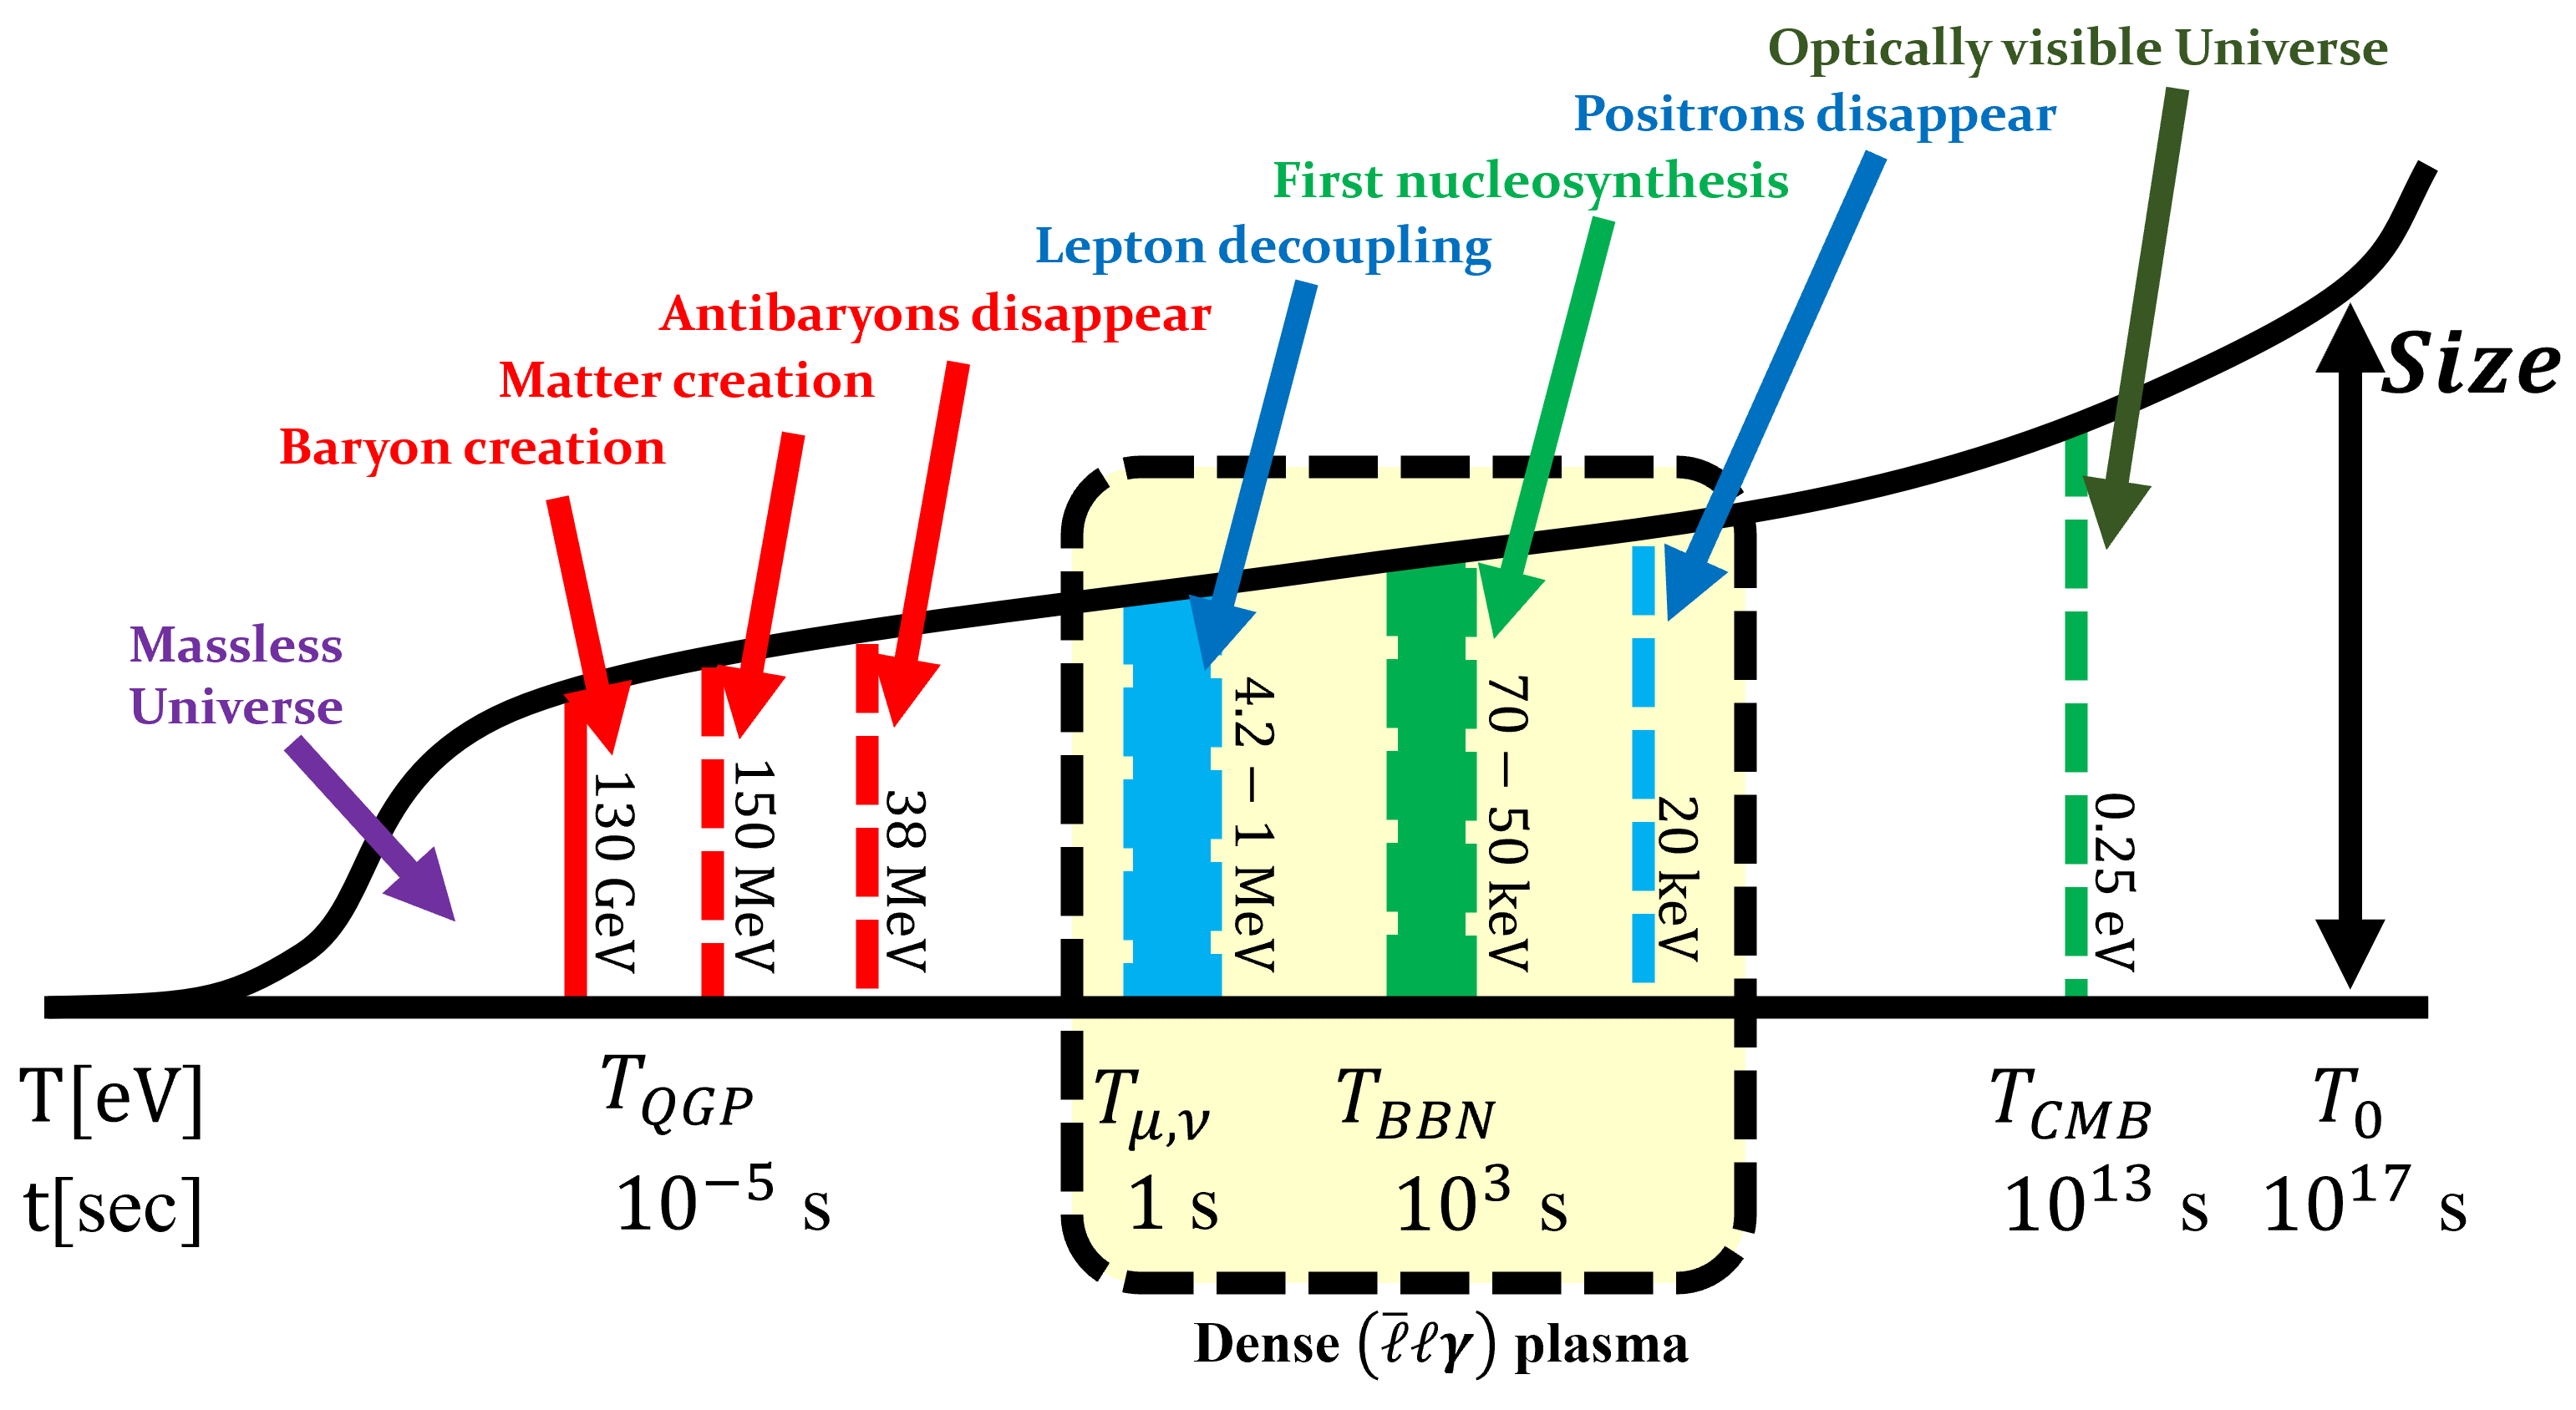
\includegraphics[width=0.95\linewidth]{plots/chap01intro/thesis_universe.png}
 \caption{A schematic of the universe's evolution since the Big Bang. The region of interest studied in this dissertation is emphasized (in the highlighted box) to contain a dense nearly charge neutral matter-antimatter plasma.}
 \label{fig:cosmo} 
\end{figure}
%%%%%%%%%%%%%%%%%%%%%%%%%%%%%%%%%%%%%%%

The scale factor $a(t)$ denotes the change of proper distances $L(t)$ over time as
\begin{gather}
    L(t)=L_{0}\frac{a_{0}}{a(t)}\rightarrow L(z)=L_{0}(1+z)\,,
\end{gather}
where $z$ is the redshift and $L_{0}$ the comoving length. In an expanding (or contracting) universe which is both homogeneous and isotropic. This implies volumes change with $V(t)=V_{0}/a^{3}(t)$ where $V_{0}=L_{0}^{3}$ is the comoving Cartesian volume. The evolutionary expansion of the universe is then traditionally defined in terms of the Hubble parameter $H(t)$ following the conventions in~\cite{weinberg1972gravitation}
\begin{gather}
  \label{Friedmann:1} H(t)^{2}\equiv\left(\frac{\dot a}{a}\right)^2=\frac{8\pi G_{N}}{3}\rho_\mathrm{total},\qquad \rho_\mathrm{total}(t)=\rho_{\Lambda}+\rho_\mathrm{DM}(t)+\rho_\mathrm{Baryons}(t)+\ldots\\
  \label{Friedmann:2}
  \frac{\ddot a}{a}=-qH^2,\qquad 
q\equiv -\frac{a\ddot a}{\dot a^2},\qquad \dot H=-H^2(1+q).
\end{gather}
where $G_N$ is the Newtonian constant of gravitation. \req{Friedmann:1} and \req{Friedmann:2} are also known as the Friedmann equations. The total density $\rho_\mathrm{total}$ is the sum of all contributions from any form of matter, radiation or field. This includes but is not limited to: dark energy $(\Lambda)$, dark matter (DM), baryons (B), leptons $(\ell,\nu)$ and photons $(\gamma)$. Depending on the age of the universe, the relative importance of each group changes as each dilutes differently under expansion with dark energy infamously remaining constant in density and accelerating the universe today.

The parameter $q$ is the cosmic deceleration which for historical reasons is positive $q>0$ under deceleration. This convention was chosen before the discovery of dark energy under the tacit assumption that the universe would be decelerating. The value of $q$ depends on energy content: The early universe was radiation dominated $(q = 1)$, subsequently matter dominated $(q = 1/2)$, and lastly the contemporary universe is undergoing a transition from matter to dark energy dominated approaching the asymptotic value of $q = -1$; see~\cite{Rafelski:2013yka}.

We can consider the expansion to be an adiabatic process~\cite{Abdalla:2022yfr} which results in a smooth shifting of the relevant dynamical quantities. As the universe undergoes isotropic expansion, the temperature decreases as 
\begin{gather}
 \label{tscale}
 T(t)=T_{0}\frac{a_{0}}{a(t)}\rightarrow T(z)=T_{0}(1+z)\,,
\end{gather}
where $z$ is the redshift. The entropy within a comoving volume is kept constant until gravitational collapse effects become relevant. The comoving temperature $T_{0}$ is given by the the present CMB temperature $T_{0}=2.7{\rm\ K}\simeq2.3\times10^{-4}\eV$~\cite{Planck:2018vyg}, with contemporary scale factor $a_{0}=1$.

As the universe expands, redshift reduces the momenta of particles lowering their contribution to the energy content of the universe. This cosmic redshift is written as
\begin{alignat}{1}
  \label{Redshift} p_{i}(t) = p_{i,0}\frac{a_{0}}{a(t)}\,.
\end{alignat}
Momentum (and the energy of massless particles $E=pc$) scales with the same factor as temperature. The energy of massive free particles in the universe however scales differently based on their momentum (and thus temperature).

When hot and relativistic, particle energy decreases inversely with scale factor like radiation. As the particles transition to non-relativistic (NR) energies, they decrease with the inverse square of the scale factor
\begin{alignat}{1}
    \label{EScale} E(t) = E_{0}\frac{a_{0}}{a(t)}\xrightarrow{\mathrm{NR}}\  E_{0}\frac{a_{0}^{2}}{a(t)^{2}}\,.
\end{alignat}
This occurs because of the functional dependence of energy on momentum in the relativistic $E\sim p$ versus non-relativistic $E\sim p^{2}$ cases.